\documentclass{ltjsarticle} %lualatex cs_jikken.texで作成 
\usepackage{mdframed}
\usepackage{graphicx}
\usepackage{float}
\usepackage{array}
\usepackage{tikz}
\usepackage{circuitikz}
\usetikzlibrary{automata, positioning, arrows}
\begin{document}

\thispagestyle{empty}
\begin{flushright}
{\large 実験実施日 2024年10月17日, 24日{\hspace{5cm}}} 
\end{flushright}

\vspace*{\fill}
\centering
{\Huge\bf コンピュータ科学実験b}
\vspace*{1cm}

{\huge\bf ハードウェア Raspberry Pi による制御}
\vspace*{\fill}

\vspace*{\fill}

\vspace*{\fill}

\begin{flushright}
{\large 学生番号: 102210017} \\ % 5cmの空白を作り、アンダーラインを引く
{\large 氏名: 安藤駿} \\
\end{flushright}

\clearpage

\addtocounter{page}{-1}
\raggedright
\setlength{\parindent}{1em}

\section{はじめに}
これまで様々なモノは個別に役割を果たしていたが, モノにセンサやアクチュエータを搭載し, インターネ
ットに接続可能とすることで, 現実世界の様々な情報収集, モノの遠隔制御, モノ同⼠の相互作⽤が可能とな
る. この考え⽅がIoT(Internet of Things)である. Raspberry Piを⽤いてIoTのデバイス管理を
体験, 学習する. Raspberry Piを⽤いたLED, スイッチ, ステッピングモータの制御を⾏う.


\section{課題3  マニュアル操作ステッピングモータカーの作成}

\subsection{目的・概要}
Raspberry Pi を⽤いて5つのボタンにより, 前進, 後退, 左回転, 右回転, 停⽌が制御可能な
敷設コースを⾛破可能なステッピングモータカーを作成する. 

\subsection{必要な部品}

\subsubsection{Raspberry Piとその他部品}
• Raspberry Pi 3 model B+

• Micro SDカード(Raspberry Pi OS 書き込み済み)

• HDMIケーブル

• Micro USB電源ケーブル

• モニタ

実験室のモニタと自宅のモニタを使用した.

• USBキーボード

使用する製品は, SANWA社のSKB-KG3WNである. シリアル番号は, 20200500196である. 

• USBマウス

使用する製品は, ELECOM社のM-K6URBK/RSである. シリアル番号は, 1203314Cである. 


\subsubsection{ブレッドボード}
ブレッドボードは電⼦回路の試作に使⽤される. 電⼦部品の端⼦を差し込む⽳が多数存在し, それぞれの⽳
に差し込んだ端⼦が接続される.この接続関係を考慮して部品を配置することで, はんだ
付けを⾏うことなく電⼦回路を組むことができる.

\subsubsection{GPIOブレッドボード接続ケーブル}
Raspberry Pi の GPIOをブレッドボードへ接続することで, 部品の配線が容易となる.

\subsubsection{押しボタンスイッチ}
2種類の端⼦を持ち, ボタンが押された間は2端⼦が導通状態, ボタンが押され
ていない間は解放状態となる.

\subsubsection{抵抗(1kΩ)}
金属皮膜抵抗1kΩ

\subsubsection{配線ケーブル}
オス-オス, メス-オスを使用した.

\subsubsection{ステッピングモータ}
モータの各相(コイル)に,ある順序で励磁パルスを与えると⼀定⾓度回転する. 

\subsubsection{ステッピングモータ制御回路}
モータをあらかじめ設定した励磁⽅式に従って電流を流すように制御する. 

\subsubsection{2.1mm DCジャック}
USB DC5V to DC12V 昇圧ケーブルを接続し, モバイルバッテリーを使う. 

\subsubsection{USB DC5V to DC12V 昇圧ケーブル}
モバイルバッテリーとDCジャックを接続する. 

\subsubsection{モバイルバッテリー}
ELECOM社のEC-M01BKを使用した. 

\subsubsection{構築部材}
ステッピングモータマウンタや従輪の構築部材にレゴを⽤いた.  

\subsection{実験方法}
表\ref{tab:tab3}のように, ステッピングモータ, テッピングモータ制御回路, 抵抗, 押しボタンスイッチ, 
DCジャックを配置した. 

\begin{table}[H] % ここで[h]は表の位置をこの場所にすることを指定します
  \centering % 表を中央に配置
  \caption{回路の接続方法}
  \begin{tabular}{|c|c|c|} 
  \hline % 上の横線
  接続する部品 & 接続1 & 接続2 \\ \hline % 行の内容と行間の横線
  抵抗とSWITCH1 & GPIO5 & GND \\ \hline
  抵抗とSWITCH2 & GPIO23 & GND \\ \hline
  抵抗とSWITCH3 & GPIO16 & GND \\ \hline
  抵抗とSWITCH4 & GPIO20 & GND \\ \hline
  抵抗とSWITCH5 & GPIO21 & GND \\ \hline
  モータ制御回路1 IN 1 & GPIO6 &   \\ \hline
  モータ制御回路1 IN 2 & GPIO13 &  \\ \hline
  モータ制御回路1 IN 3 & GPIO19 &  \\ \hline
  モータ制御回路1 IN 4 & GPIO26 &  \\ \hline
  モータ制御回路1 + & DCジャック + & \\ \hline
  モータ制御回路1 - & DCジャック - & \\ \hline
  モータ制御回路2 IN 1 & GPIO4 &   \\ \hline
  モータ制御回路2 IN 2 & GPIO17 &  \\ \hline
  モータ制御回路2 IN 3 & GPIO27 &  \\ \hline
  モータ制御回路2 IN 4 & GPIO22 &  \\ \hline
  モータ制御回路2 + & DCジャック + & \\ \hline
  モータ制御回路2 - & DCジャック - & \\ \hline
  DCジャック -  & GND & \\ \hline

  \end{tabular}
  \label{tab:tab3} % 表を参照するためのラベル
\end{table}

レゴを用いて, マウンタ, Raspberry Pi, ブレッドボード, モバイルバッテリーを搭載したステッピングモータカーを作成した. 
これを図\ref{fig:raspi3}に示す. 

このマニュアル操作モータカーを動かすためのコード3.pyを作成した. これを図\ref{fig:3py}に示す. 
スイッチ1が前進, スイッチ2が左旋回, スイッチ3が右旋回, スイッチ4が後退, スイッチ5が停止に対応している. 

コースの入り口にステッピングモータカーを置き, 作成した3.pyを実行した. 
そして, コースの状況に合わせてスイッチを押し, 前進, 右折, 左折, 後退, 停止をさせ, 出口までモーターカーを走らせた. 
使用するコースを図\ref{fig:road}に示す. 


\begin{figure}[H] % 画像を挿入する環境を開始
  \centering
  \begin{minipage}{0.45\textwidth} % 1つ目の画像の幅をページの45%に設定
    \centering
    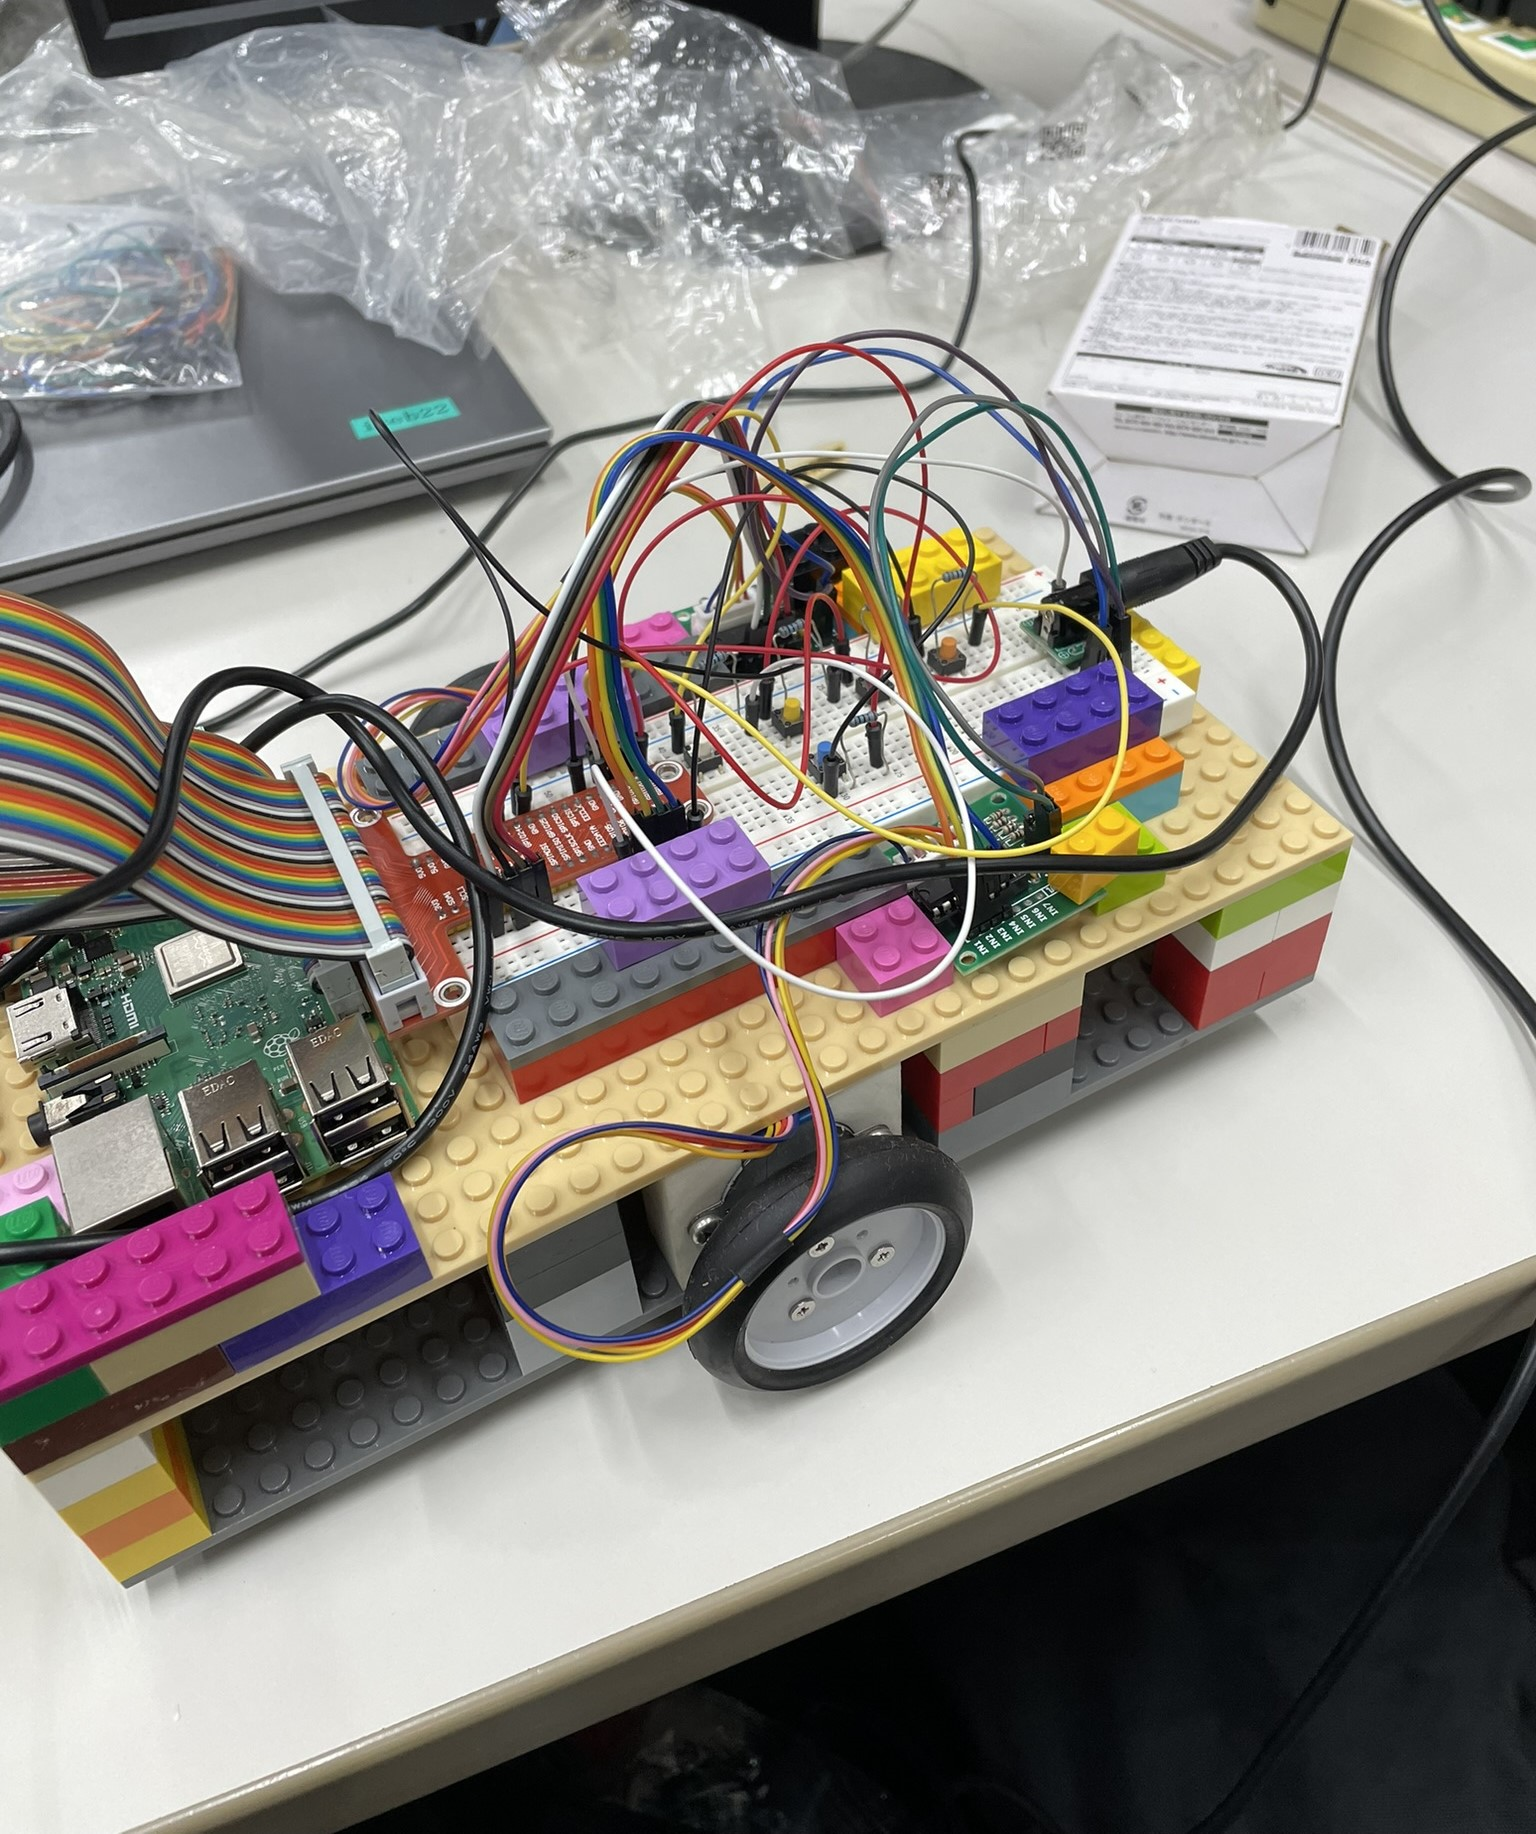
\includegraphics[width=\textwidth]{raspi3.JPEG} % 画像を挿入、幅をminipage幅に合わせる
    \caption{作成したステッピングモータカー} % キャプションを追加
    \label{fig:raspi3} % ラベルを追加
  \end{minipage}
  \hfill % 画像の間にスペースを追加
  \begin{minipage}{0.45\textwidth} % 2つ目の画像の幅をページの45%に設定
    \centering
    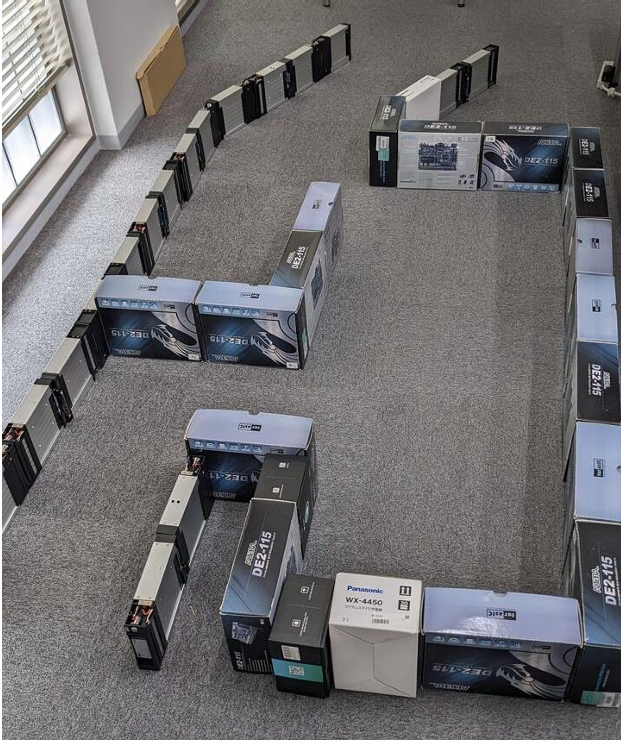
\includegraphics[width=\textwidth]{road.png} % 2つ目の画像を挿入
    \caption{使用するコース} % キャプションを追加
    \label{fig:road} % ラベルを追加
  \end{minipage}
\end{figure}


\begin{mdframed}
  \begin{verbatim}
    //省略

    isForward=False
    isBack=False
    isStopped=False
    isTurnRight=False
    isTurnLeft=False

    i = 0 #モーター1
    j = 0 #モーター2
    while True:
        # スイッチ1接続端⼦の状態読み取り
        if switch1.value == 1:
            isForward = True 
            isBack=False
            isTurnRight=False
            isTurnLeft=False       
            print("Switch1 on")
            time.sleep(1)

        # スイッチ2接続端⼦の状態読み取り    
        if switch2.value == 1:
            isForward = False 
            isBack=True
            isTurnRight=False
            isTurnLeft=False     
            print("Switch2 on")
            time.sleep(1)

        # スイッチ3接続端⼦の状態読み取り
        if switch3.value == 1: 
            isForward = False
            isBack=False 
            isTurnLeft=False
            isTurnRight=True           
            print("Switch3 on")
            time.sleep(1)

        # スイッチ4接続端⼦の状態読み取り    
        if switch4.value == 1: 
            isForward = False
            isBack=False 
            isTurnLeft=True
            isTurnRight=False    
            print("Switch4 on")
            time.sleep(1)   

        # スイッチ5接続端⼦の状態読み取り    
        if switch5.value == 1: 
            if(isStopped == False):
                isStopped = True 
            else:
                isStopped = False   
            print("Switch5 on")
            time.sleep(1)       

        if isStopped == True:
            time.sleep(1)
        else:
            if(isForward == True):
                i += 1
                if i >= 4:
                    i = 0
                j -=1
                if j <= -1:
                    j = 3

            if(isBack == True):
                i -= 1
                if i <= -1:
                    i = 3
                j +=1
                if j >= 4:
                    j = 0

            if(isTurnLeft):
                i += 1
                if i >= 4:
                    i = 0
                j +=1
                if j >= 4:
                    j = 0

            if(isTurnRight):
                i -= 1
                if i <= -1:
                    i = 3
                j -=1
                if j <= -1:
                    j = 3      
                          
            out_motor1_pin(i)
            out_motor2_pin(j)
            # 乱調を避けるために少し待つ
            time.sleep(TIME_SLEEP)	
  \end{verbatim}
  \end{mdframed}
  \begin{figure}[H]
  \caption{3.pyの一部}
  \label{fig:3py}
\end{figure}
 

\subsection{実験結果}
3.pyを実行しスイッチ1を押した結果, ステッピングモータカーが前進した. 
一つ目の右折でスイッチ5を押した結果, モータカーが停止した. 
そして, スイッチ3を押すと, モータカーが右旋回をした. 
また, 次のT字路にて, スイッチ5で停止させた後スイッチ2を押すと, 左旋回をした. 
このように, コースに合わせてスイッチを押した結果, 走破することができた. 
提出した課題3.MP4にこのときの状況が記録されている. 


\subsection{考察}
各スイッチに対し一つずつbooleanの値を用いたことで, 5つの状態を正しく管理することができた. 
これは, 課題2-5で作成したコードと原理は同じと考えられる.  

初めにモータのタイヤをステッピングモータカーの後部に設置し, 前部には別のタイヤを設置したところ, 絨毯の上でうまく旋回しなかった. 
そこで, モータのタイヤを真ん中に設置し別のタイヤを使わないようにした結果, うまく旋回するようになった. 
これはステッピングモータのタイヤのみに力がかかるようになり, 余計な摩擦が減ったからだと考えられる. 
  


\section{課題4  ⾃動⾛⾏ステッピングモータカーの作成}

\subsection{目的・概要}
Raspberry Pi と距離センサ計を⽤いて, 1つ以上のT字路, 右折, 左折路を含むコースを⾃動で⾛破可能なステッピ
ングモータカーを作成する. 

\subsection{必要な部品}

\subsubsection{課題3と同じ部品}
Raspberry Pi とその他部品, ブレッドボード, GPIO ブレッドボード接続ケーブル, 配線ケーブル, 
ステッピングモータ, ステッピングモータ制御回路, 2.1mm DC ジャック, USB DC5V to DC12V 昇圧ケーブル, 
モバイルバッテリー, 構築部材は課題3と同じ部品を使用した. 

\subsubsection{⾚外線式距離センサ計: Sharp GP2YOA21}
80cm程度までの距離を計測でき, 距離に応じた電圧(約0.5-3.2V)を出⼒する. 

\subsubsection{A/Dコンバータ: MCP3424 with address switch}
アナログ信号の振幅を離散的な周期で切り出し, 符号で表されたデジタル信号に変換する. 
標本化, 量子化, 符号化の順にデジタル信号に変換していく. 

標本化は, 連続なアナログ信号の振幅値を離散的な周期で切り出すことである. 
量子化は, 離散的な周期で切り出された振幅値を、離散的な振幅値に近似することである. 
符号化は, 離散的な振幅値を"0"と"1"の2値で表す符号に変換することである. 
(rohm, 2024)

\subsubsection{抵抗(1MΩ)}
金属皮膜抵抗1MΩ
 

\subsection{実験方法}
表\ref{tab:tab4}, 図\ref{fig:fig4}に示すように, ステッピングモータ, テッピングモータ制御回路, 抵抗, 
DCジャック, GP2Y0A21, MCP3424を配置した. 

\begin{table}[H] % ここで[h]は表の位置をこの場所にすることを指定します
  \centering % 表を中央に配置
  \caption{回路の接続方法}
  \begin{tabular}{|c|c|c|} 
  \hline % 上の横線
  接続する部品 & 接続1 & 接続2 \\ \hline % 行の内容と行間の横線
  モータ制御回路1 IN 1 & GPIO6 &   \\ \hline
  モータ制御回路1 IN 2 & GPIO13 &  \\ \hline
  モータ制御回路1 IN 3 & GPIO19 &  \\ \hline
  モータ制御回路1 IN 4 & GPIO26 &  \\ \hline
  モータ制御回路2 IN 1 & GPIO4 &   \\ \hline
  モータ制御回路2 IN 2 & GPIO17 &  \\ \hline
  モータ制御回路2 IN 3 & GPIO27 &  \\ \hline
  モータ制御回路2 IN 4 & GPIO22 &  \\ \hline
  モータ制御回路1, 2 + & DCジャック + & \\ \hline
  モータ制御回路1, 2 - & DCジャック - & \\ \hline
  DCジャック -  & GND & \\ \hline
  1MΩ抵抗1 & GP2YOA21 1 vo & MCP3424 ch1+ \\ \hline
  1MΩ抵抗2 & GP2YOA21 2 vo & MCP3424 ch2+ \\ \hline
  1MΩ抵抗3 & GP2YOA21 3 vo & MCP3424 ch3+ \\ \hline
  MCP3424 ch1-,ch2-,ch3- & GND &  \\ \hline
  MCP3424 +5v & 5v &  \\ \hline
  MCP3424 GND & GND &  \\ \hline
  MCP3424 SDA & SDA1 &  \\ \hline
  MCP3424 SCL & SCL1 &  \\ \hline
  GP2YOA21 1,2,3 GND & GND &  \\ \hline
  GP2YOA21 1,2,3 Vcc & 5v &  \\ \hline 
  
  \end{tabular}
  \label{tab:tab4} % 表を参照するためのラベル
\end{table}

課題3で作成したステッピングモータカーにレゴを用いてGP2YOA21を設置した. 
これを図\ref{fig:raspi4-1}, 図\ref{fig:raspi4-2}に示す.  

この⾃動⾛⾏ステッピングモータカーを図\ref{fig:road}のコースに対し, 順走させるためのコード4-1.pyと逆走させるためのコード4-2.pyを作成した. 
これらを図\ref{fig:4-1py}, \ref{fig:4-2py}に示す. 

コースの入口にステッピングモータカーを置き, 作成した4-1.pyを実行した. 
その後, コースの出口にステッピングモータカーを置き, 作成した4-2.pyを実行した. 

\begin{figure}[H] % 画像を挿入する環境を開始
  \centering
  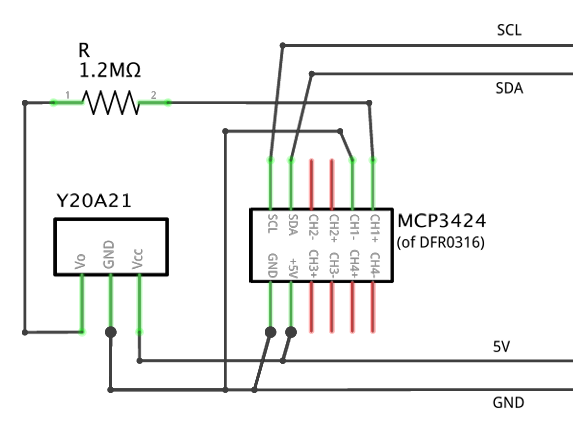
\includegraphics[width=0.5\textwidth]{fig4.png} % 画像を挿入、幅をページ幅に合わせる
  \caption{GP2Y0A21とMCP3424を⽤いた距離計測回路} % キャプションを追加
  \label{fig:fig4} % ラベルを追加
\end{figure}

\begin{figure}[H] % 画像を挿入する環境を開始
  \centering
  \begin{minipage}{0.45\textwidth} % 1つ目の画像の幅をページの45%に設定
    \centering
    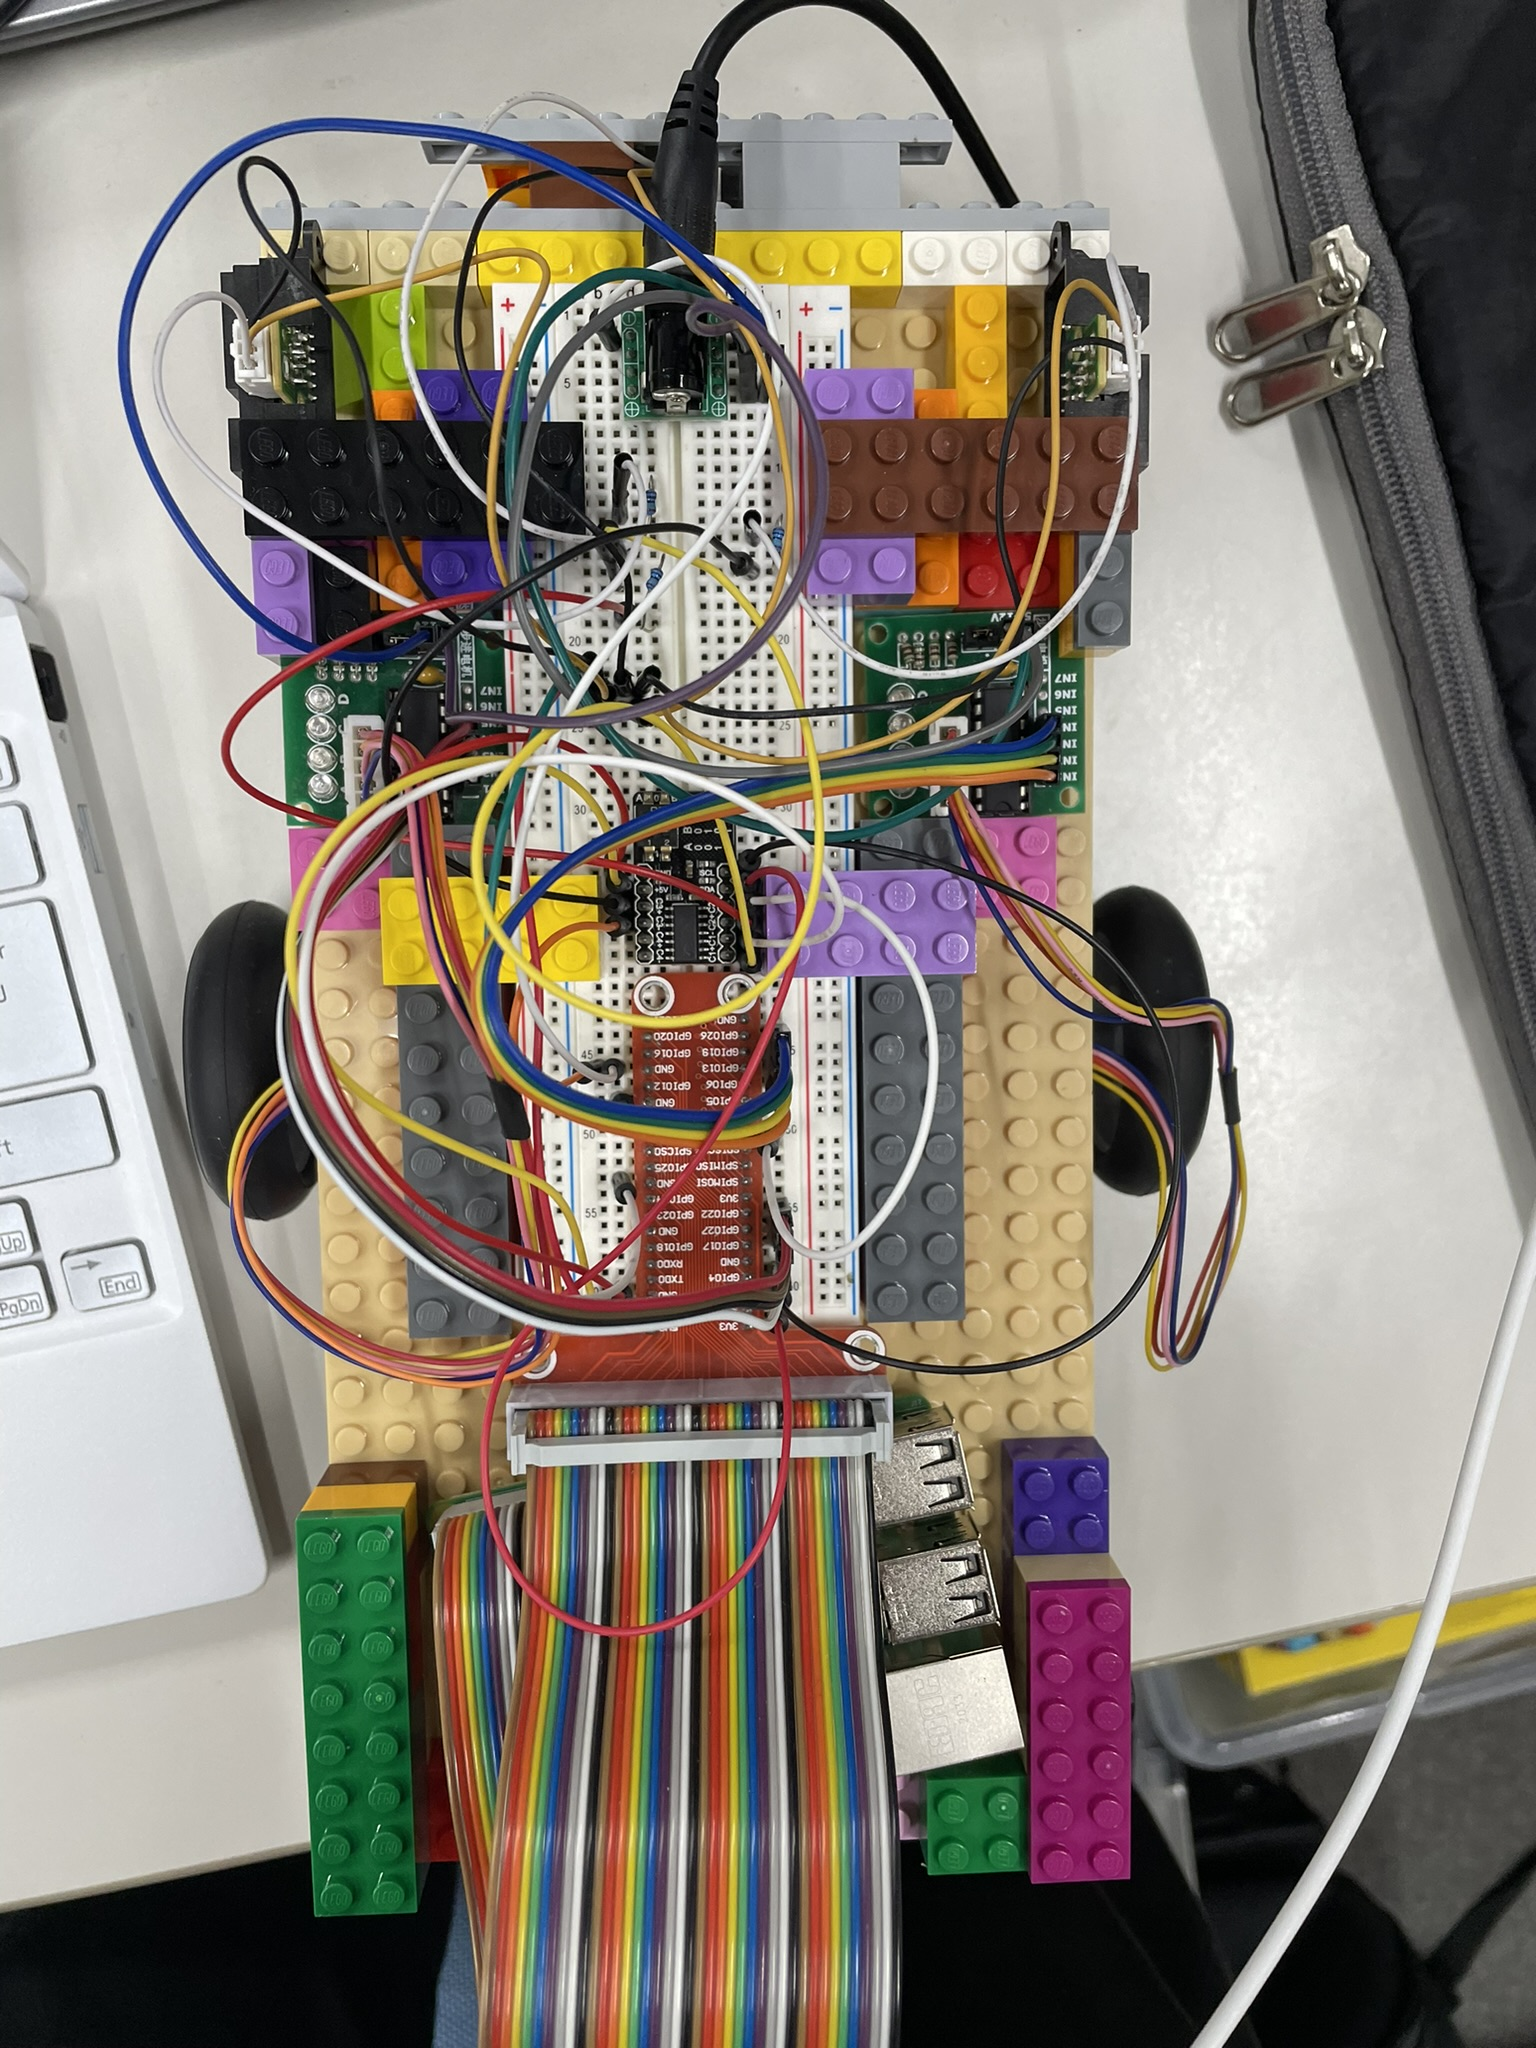
\includegraphics[width=\textwidth]{raspi4-1.JPEG} % 画像を挿入、幅をminipage幅に合わせる
    \caption{作成したステッピングモータカー} % キャプションを追加
    \label{fig:raspi4-1} % ラベルを追加
  \end{minipage}
  \hfill % 画像の間にスペースを追加
  \begin{minipage}{0.45\textwidth} % 2つ目の画像の幅をページの45%に設定
    \centering
    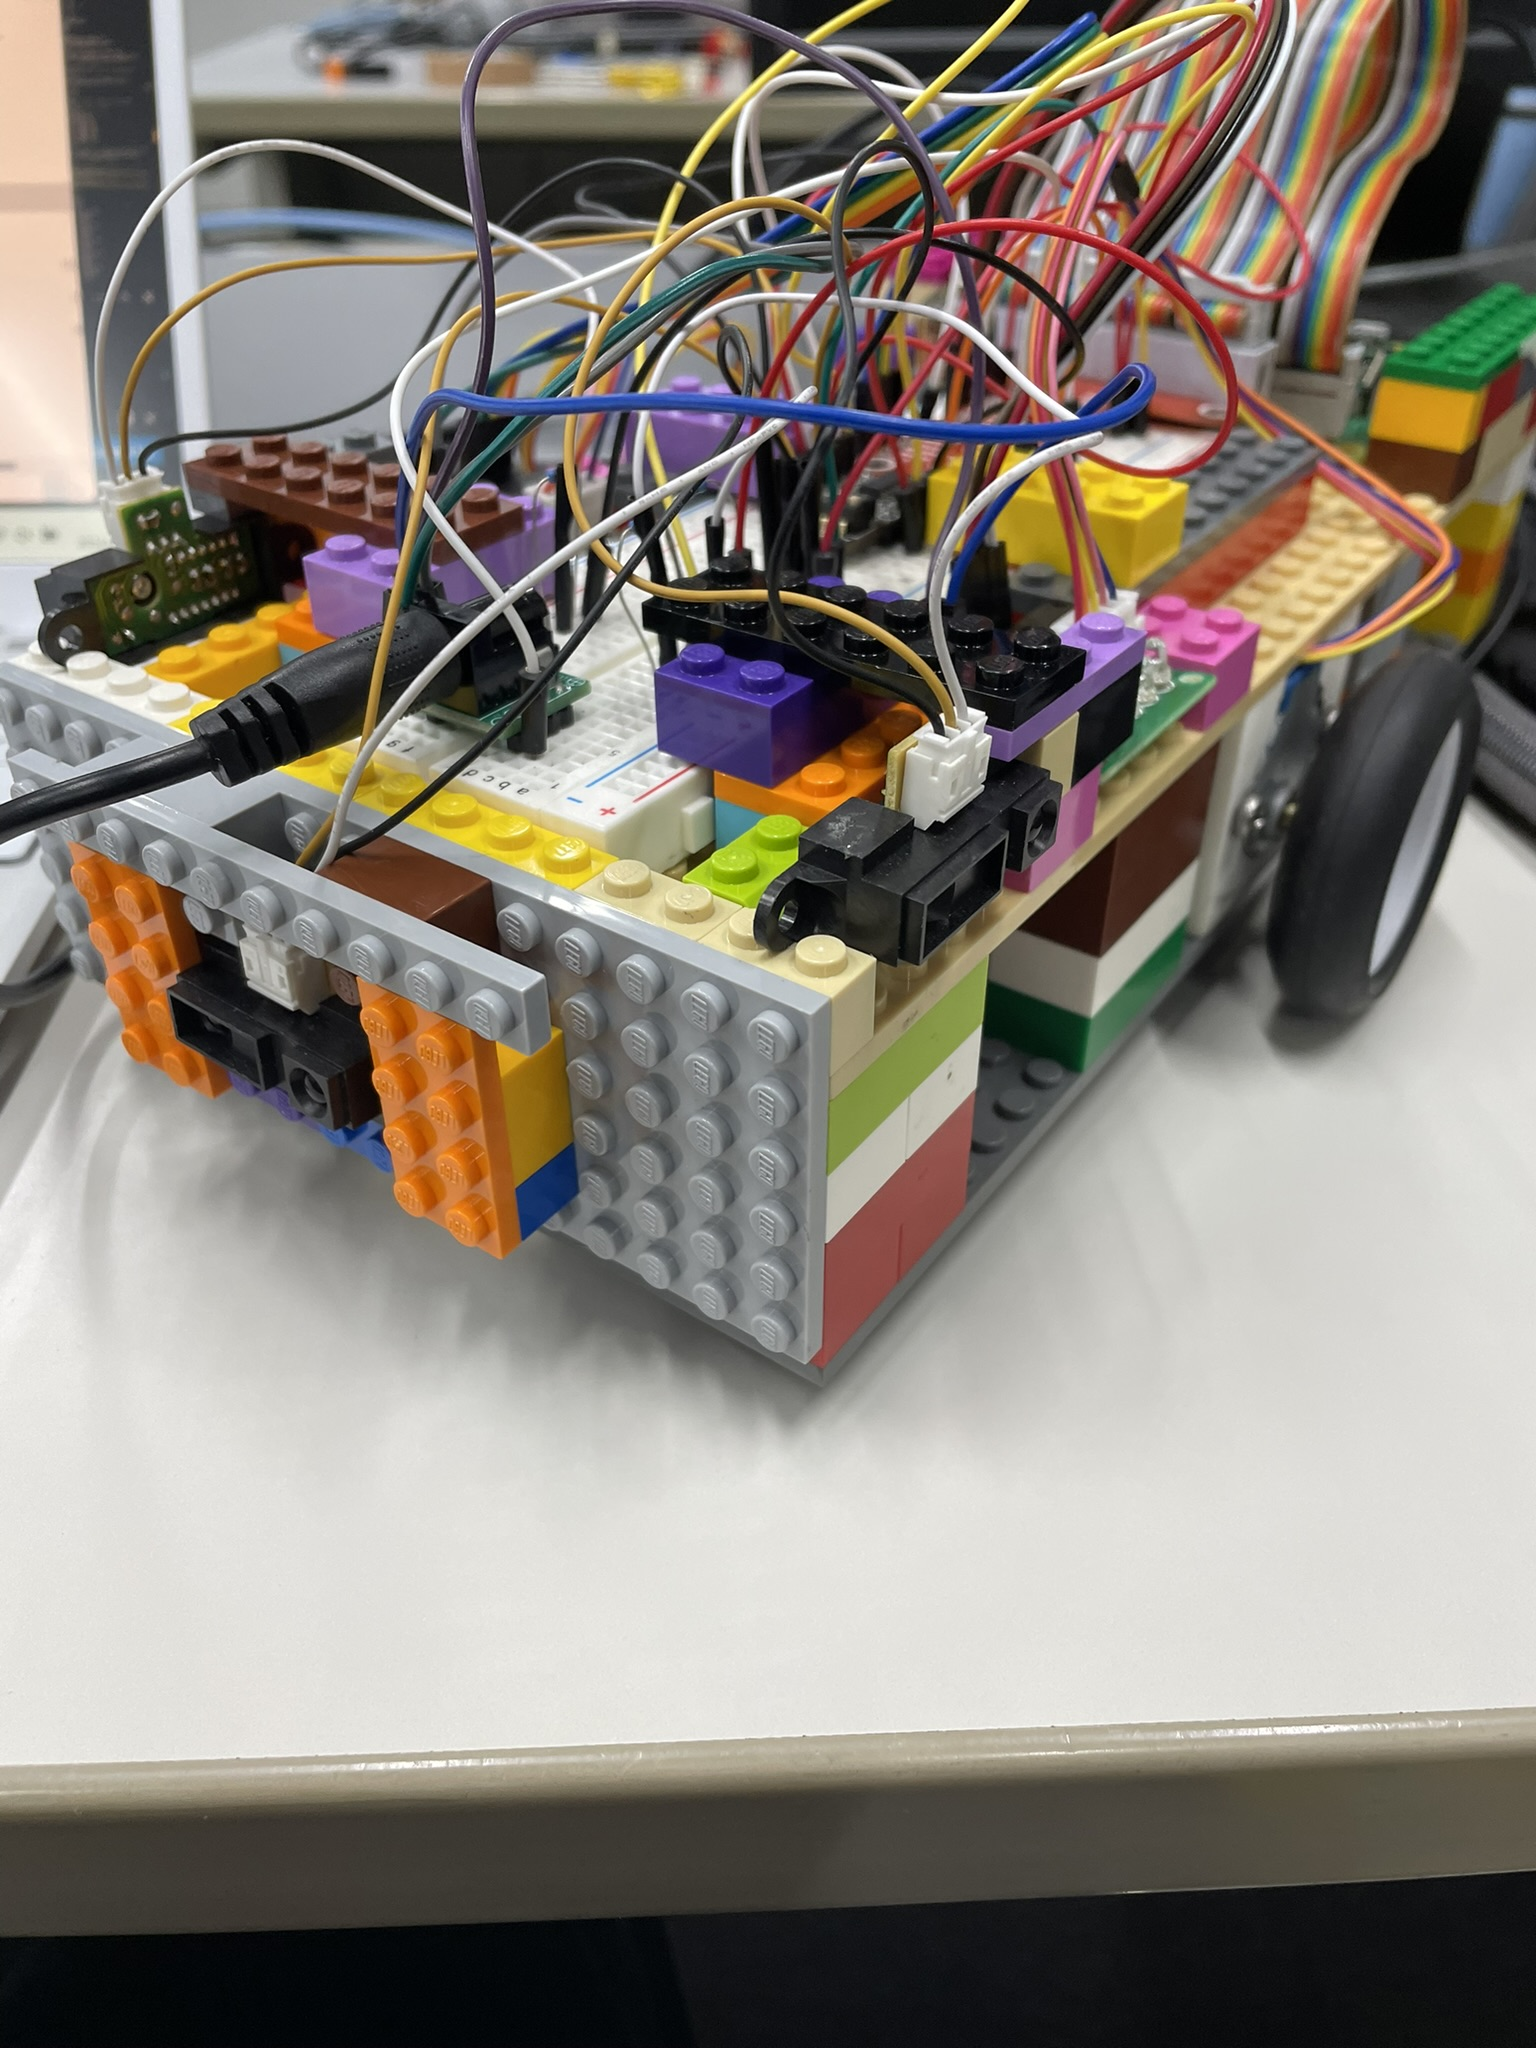
\includegraphics[width=\textwidth]{raspi4-2.JPEG} % 2つ目の画像を挿入
    \caption{作成したステッピングモータカー} % キャプションを追加
    \label{fig:raspi4-2} % ラベルを追加
  \end{minipage}
\end{figure}


\begin{mdframed}
  \begin{verbatim}
    //省略

    i = 0 #モーター1
    j = 0 #モーター2
    k = 0 #時間管理用
    isForward = False
    isTurnRight=False
    isTurnLeft=False
    while True:
        k += 1
        if(k%200==0):
            config1 = (mcp3424.cfg_read | mcp3424.cfg_ch1 | mcp3424.cfg_once |
                    mcp3424.cfg_12bit | mcp3424.cfg_PGAx1)
            config2 = (mcp3424.cfg_read | mcp3424.cfg_ch2 | mcp3424.cfg_once |
                    mcp3424.cfg_12bit | mcp3424.cfg_PGAx1)
            config3 = (mcp3424.cfg_read | mcp3424.cfg_ch3 | mcp3424.cfg_once |
                    mcp3424.cfg_12bit | mcp3424.cfg_PGAx1)
            
            # ch1
            data1 = i2c.write_byte(addr, config1)
            time.sleep(1 / mcp3424.sps_12bit)
            while True:
                data1 = i2c.read_i2c_block_data(addr, 0, 3)  # Read the current value
                if data1[2] >> 7 == 0:
                    break
                time.sleep(0.001)
            volt1 = mcp3424.to_volt(data1, 12)    
    
            # ch2
            data2 = i2c.write_byte(addr, config2)
            time.sleep(1 / mcp3424.sps_12bit)
            while True:
                data2 = i2c.read_i2c_block_data(addr, 0, 3)  # Read the current value
                if data2[2] >> 7 == 0:
                    break
                time.sleep(0.001)
            volt2 = mcp3424.to_volt(data2, 12)    
    
            # ch3
            data3 = i2c.write_byte(addr, config3)
            time.sleep(1 / mcp3424.sps_12bit)
            while True:
                data3 = i2c.read_i2c_block_data(addr, 0, 3)  # Read the current value
                if data3[2] >> 7 == 0:
                    break
                time.sleep(0.001)        
            volt3 = mcp3424.to_volt(data3, 12)
            print("ch1:"+ str(volt1) + "ch2:"+ str(volt2) + "ch3:"+ str(volt3))
    
            if volt2 < 1.0:
                isForward = True
                isTurnRight=False
                isTurnLeft=False
            elif volt1 > volt3:
                isForward = False
                isTurnRight=True
                isTurnLeft=False
            else:
                isForward = False
                isTurnRight=False
                isTurnLeft=True    
    
            if volt1 > 1.7:
                isForward = False
                isTurnRight=True
                isTurnLeft=False
            if volt3 > 1.7:
                isForward = False
                isTurnRight=False
                isTurnLeft=True   
    
        #print(isForward)    
        if(isForward == True):
            i += 1
            if i >= 4:
                i = 0
            j -=1
            if j <= -1:
                j = 3    
    
        if(isTurnRight):
            i -= 1
            if i <= -1:
                i = 3
            j -=1
            if j <= -1:
                j = 3  
    
        if(isTurnLeft):
            i += 1
            if i >= 4:
                i = 0
            j +=1
            if j >= 4:
                j = 0
                          
        out_motor1_pin(i)
        out_motor2_pin(j)
        # 乱調を避けるために少し待つ
        time.sleep(TIME_SLEEP) 	
  \end{verbatim}
  \end{mdframed}
  \begin{figure}[H]
  \caption{4-1.pyの一部}
  \label{fig:4-1py}
\end{figure}


\begin{mdframed}
  \begin{verbatim}
    //省略

        if volt2 < 1.5:
            if volt3 < 1.5 and volt3 > 0.8:
                isForward = True
                isTurnRight=False
                isTurnLeft=False
            elif volt3 > 1.5:
                
                isForward = False
                isTurnRight=False
                isTurnLeft=True
            else:
                print("go straight\n")
                for l in range(500):                    
                    i += 1
                    if i >= 4:
                        i = 0
                    j -=1
                    if j <= -1:
                        j = 3
                    out_motor1_pin(i)
                    out_motor2_pin(j)
                    # 乱調を避けるために少し待つ
                    time.sleep(TIME_SLEEP)
                isForward = False
                isTurnRight=True
                isTurnLeft=False

        if volt2 > 1.0:
            if volt1 > volt3:
                print("turn right\n")
                for l in range(800):                    
                    i -= 1
                    if i <= -1:
                        i = 3
                    j -=1
                    if j <= -1:
                        j = 3
                    out_motor1_pin(i)
                    out_motor2_pin(j)
                    # 乱調を避けるために少し待つ
                    time.sleep(TIME_SLEEP) 
            else:
                print("turn left\n")
                for l in range(800):                    
                    i += 1
                    if i >= 4:
                        i = 0
                    j +=1
                    if j >= 4:
                        j = 0
                    out_motor1_pin(i)
                    out_motor2_pin(j)
                    # 乱調を避けるために少し待つ
                    time.sleep(TIME_SLEEP)        

        if volt1 > 1.7:
            isForward = False
            isTurnRight=True
            isTurnLeft=False
        if volt3 > 1.7:
            isForward = False
            isTurnRight=False
            isTurnLeft=True   

    #print(isForward)    
    if(isForward == True):
        i += 1
        if i >= 4:
            i = 0
        j -=1
        if j <= -1:
            j = 3    

    if(isTurnRight):
        i -= 1
        if i <= -1:
            i = 3
        j -=1
        if j <= -1:
            j = 3  

    if(isTurnLeft):
        i += 1
        if i >= 4:
            i = 0
        j +=1
        if j >= 4:
            j = 0
                    
    out_motor1_pin(i)
    out_motor2_pin(j)
    # 乱調を避けるために少し待つ
    time.sleep(TIME_SLEEP)	
  \end{verbatim}
  \end{mdframed}
  \begin{figure}[H]
  \caption{4-2.pyの一部}
  \label{fig:4-2py}
\end{figure}
 

\subsection{実験結果}
4-1.pyを実行した結果, 入り口から出口まで走破した. このときの状況は課題4順走.MP4に記録されている. 
一つ目のT字路では左折し最短経路を通ったが, 二つ目のT字路では左折をして行き止まりまで進んでからUターンして出口に向かった. 

4-2.pyを実行した結果, 出口から入り口まで走破した. このときの状況は課題4逆走.MP4に記録されている. 
モータカーの右側の壁に沿って, コースを走行した. 


\subsection{考察}
初めにコードを作成したとき, while文内で毎ループごとにセンサーの値を受け取る設計にした. 
しかし, これではモータカーはほとんど動かなかった. 
そこでセンサーの動作を少なくするため, 毎ループごとに整数kの値を1増やしていき, 
kを200で割った余りが0になるときだけ, センサーの値を受け取るように変更した. 
この結果モータカーはうまく動いたことから, 
センサーの処理にかかる時間が大きすぎたことが原因であると考えられる. 

今回使用したGP2Y0A21とMCP3424について, 1MΩの抵抗一つを接続して使用したところ, 約20cmの距離で
1.0Vの出力があり, 約10cmの距離で1.5Vの出力があった. モータカーの前面のセンサーが1.0V以上で 
旋回するようにするとうまく機能したのは, このためであると考えられる. 

コースを順走させるには, モータカーの前方に壁が来るときに旋回をする単純なアルゴリズム(4-1.py)でよかった.  
しかし, 逆走させるにはT字路でモータカーの前方に壁がないときに旋回をしなければならない. 
そこで, モータカーの右側の壁と一定の距離を保ちながら走行するアルゴリズム(4-2.py)を考えた. 
右側のセンサーの出力が0.8Vから1.5Vになるように適宜旋回をすると, 壁との距離を10cmから15cmに保ちながら走行することができた.  
しかし, ゴールへ壁伝いで行けないコースでは, このアルゴリズムは使えないと考えられる. 


\section{まとめ}

\subsection{実験を通して分かったこと}
ステッピングモータカーの作成やGP2Y0A21とMCP3424を用いた距離計測の方法を理解した. 

\subsection{工夫したこと}
外観の美しさや環境に配慮して, ガムテープを全く使わずにステッピングモータカーを作成した. 
センサーの取り付けが特に難しかったが, 工夫してレゴを配置した. 

また, 実験で行ったことについて逐一メモや写真に記録を残し, 後から確認しやすいようにした. 

\subsection{反省点}
実験4で, 曲がり角を記憶したり地図を作成したりするような複雑なアルゴリズムではなく, その瞬間のセンサーの情報を
判断するだけの単純なアルゴリズムしか作れなかった. 
もっと創意工夫を凝らしたアルゴリズムを考えるべきだった. 


\begin{thebibliography}{99} % 最大ラベル幅を99に設定
    
  \bibitem{lamport1994latex}
  PassMark: 
  \emph{A/Dコンバータとは?}. \\
  \verb|https://www.rohm.co.jp/electronics-basics/ad-converters/ad_what2|  2024.

\end{thebibliography}


\end{document}